The architecture presented in this chapter was created following the Belief, Desires and Intentions (BDI) approach, as could be seen in the Figure~\ref{fig:GeneralArchitecture}. Additionally it was added the Description and Action modules. The first one (Description) has two goals: enable personalisation of the robot (e.g. platform and character), and describe all the necessary information to act.
\begin{figure}
	\centering
	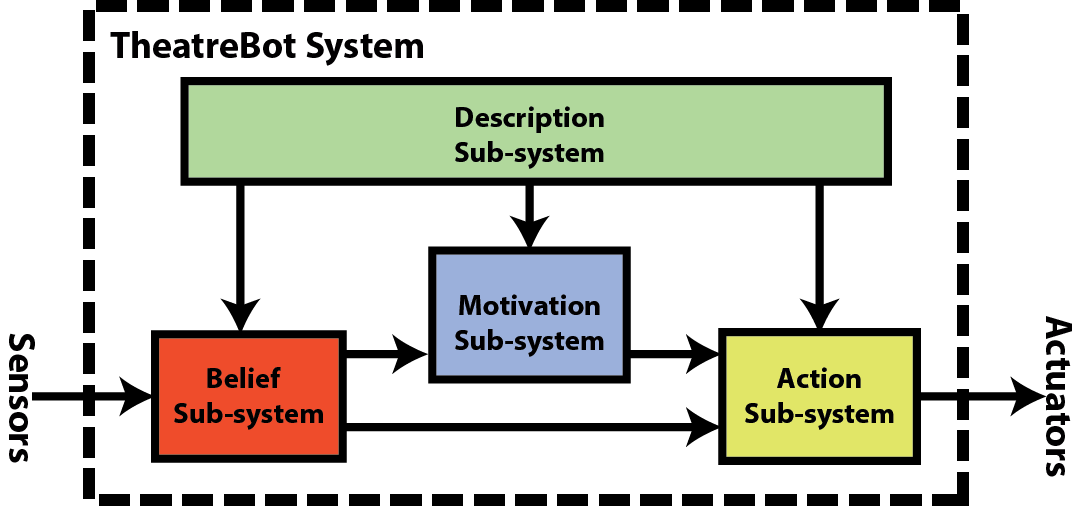
\includegraphics[width=1.0\textwidth]{./Images/Architecture/GeneralArchitecture.png} 
	\caption{General Architecture. The dash line shows the components that are in the system. The concepts of Desires and Intentions are included in the box Motivation.}
	\label{fig:GeneralArchitecture}
\end{figure}
Each of the modules are decomposed in sub-system that working as a whole could be used to accomplish the task. The final result could be seen in the Figure~\ref{fig:ArchitectureWithSubSystems}, where the module Action was divided in two: Action decision and Action modulation. Also was added the sub-module feature. Each of the modules in the architecture will be described in more detail though this chapter. 
\begin{figure}
	\centering
	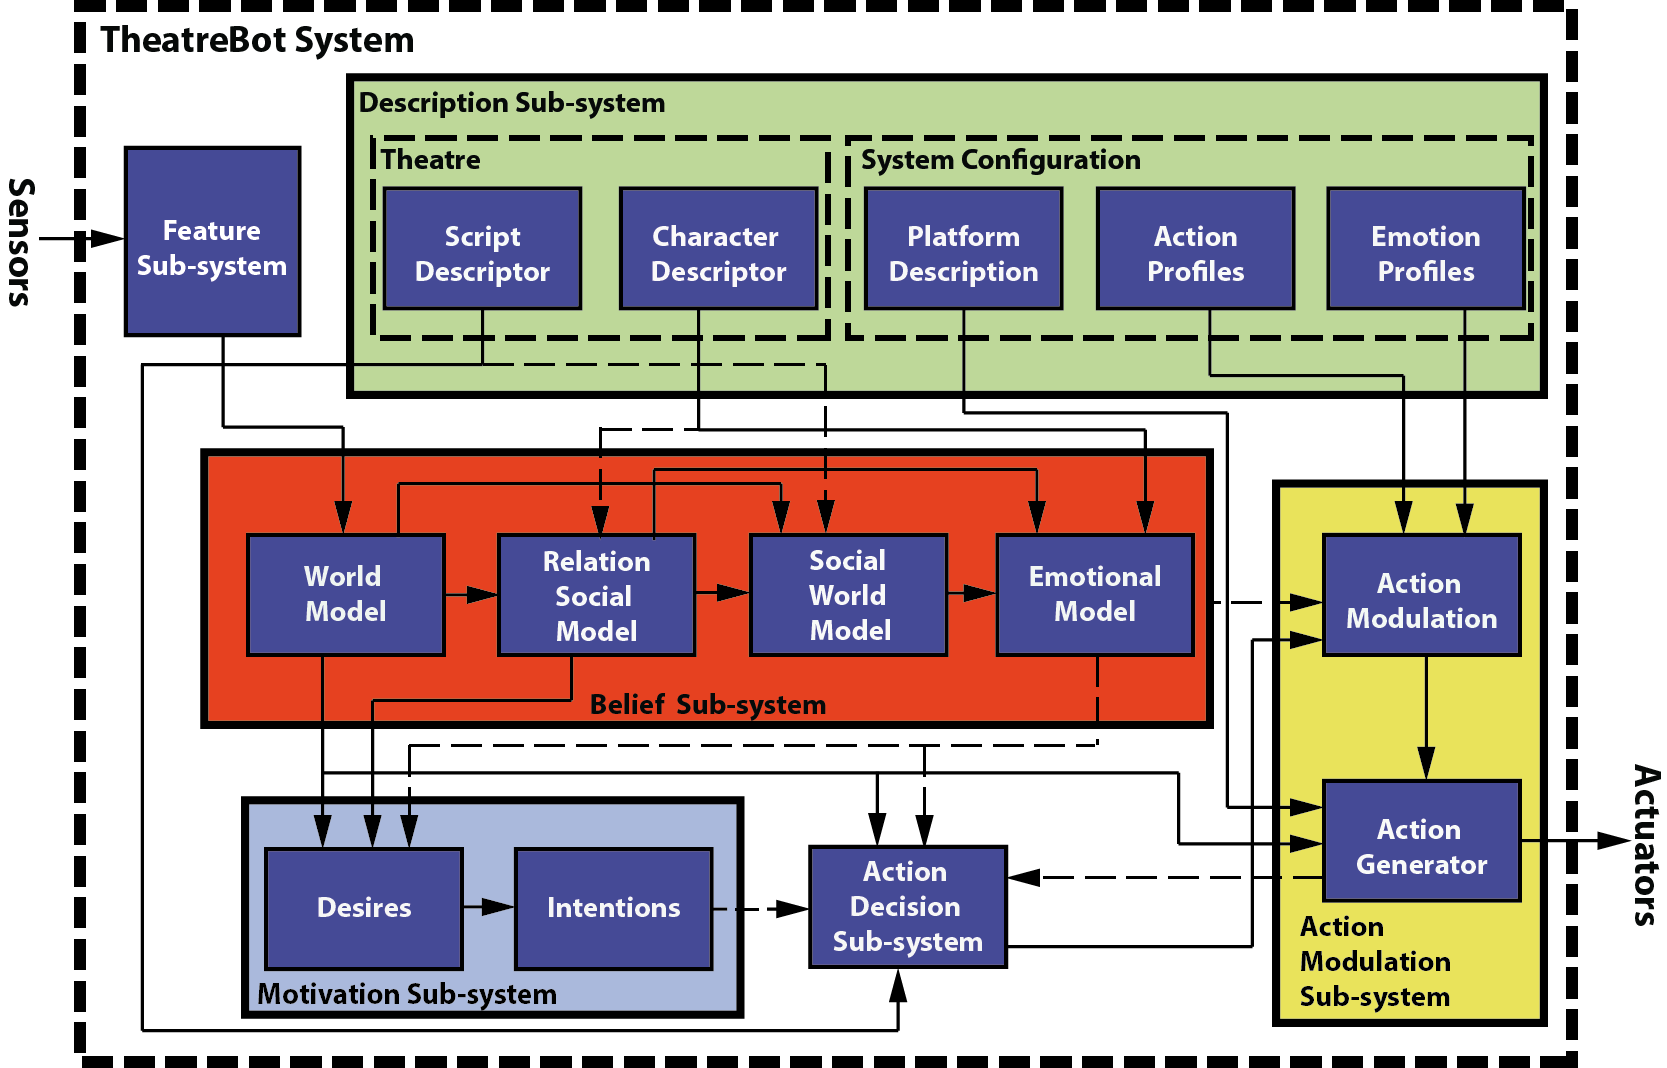
\includegraphics[width=1.0\textwidth]{./Images/Architecture/ArchitectureNew.png} 
	\caption{Architecture with the subsystems.}
	\label{fig:ArchitectureWithSubSystems}
\end{figure}



